% Template for PLoS
% Version 1.0 January 2009
%
% To compile to pdf, run:
% latex plos.template
% bibtex plos.template
% latex plos.template
% latex plos.template
% dvipdf plos.template

\documentclass[10pt]{article}

% amsmath package, useful for mathematical formulas
\usepackage{amsmath}
% amssymb package, useful for mathematical symbols
\usepackage{amssymb}

% graphicx package, useful for including eps and pdf graphics
% include graphics with the command \includegraphics
\usepackage{graphicx}

% cite package, to clean up citations in the main text. Do not remove.
\usepackage{cite}

\usepackage{color} 

% Use doublespacing - comment out for single spacing
\usepackage{setspace} 
\doublespacing

% Text layout
\topmargin 0.0cm
\oddsidemargin 0.5cm
\evensidemargin 0.5cm
\textwidth 16cm 
\textheight 21cm

% Bold the 'Figure #' in the caption and separate it with a period
% Captions will be left justified
\usepackage[labelfont=bf,labelsep=period,justification=raggedright]{caption}

% Use the PLoS provided bibtex style
\bibliographystyle{plos2009}

% Remove brackets from numbering in List of References
\makeatletter
\renewcommand{\@biblabel}[1]{\quad#1.}
\makeatother

% Leave date blank
\date{}

\pagestyle{myheadings}
%% ** EDIT HERE **
%% Please insert a running head of 30 characters or less.  
%% Include it twice, once between each set of braces
\markboth{Quantifying FA Dynamics}{Quantifying FA Dynamics}


%% ** EDIT HERE **
%% PLEASE INCLUDE ALL MACROS BELOW

%% END MACROS SECTION

\begin{document}

% Title must be 150 words or less
\begin{flushleft}
{\Large
\textbf{Automated Identification and Tracking of Focal Adhesions Reveals Phosphorylation of Paxillin at Serine 178 is a Key Regulatory Mechanism of Adhesion Assembly}
}
% Insert Author names, affiliations and corresponding author email.
\\
Matthew E. Berginski$^{1,\dagger}$, 
Eric Vitriol$^{2,\dagger}$, 
Klaus Hahn$^{3,\ast}$
Shawn M. Gomez$^{1,\ast}$
\\
\bf{1} Department of Biomedical Engineering, University of North Carolina at Chapel Hill, Chapel Hill, NC, USA
\\
\bf{2} Department of Cell and Developmental Biology, University of North Carolina at Chapel Hill, Chapel Hill, NC, USA
\\
\bf{3} Department of Pharmacology, University of North Carolina at Chapel Hill, Chapel Hill, NC, USA
\\
$\dagger$ These authors contributed equally to this work.
\\
$\ast$ To whom correspondence should be addressed. E-mail: smgomez@unc.edu (SMG); khahn@med.unc.edu (KH)
\end{flushleft}

% Please keep the abstract between 250 and 300 words
\section*{Abstract}

Focal adhesions are macromolecular complexes that provide a linkage from a cell
to its external environment. In a motile cell they form, enlarge, and
disassemble; these processes are essential to and govern cell migration. To
better understand the dynamic regulation of focal adhesions during cell motility
we have developed software for the automated detection, tracking, and data
extraction of these structures using Total Internal Reflection Fluorescence
Microscopy (TIR-FM) image sets of fluorescently tagged adhesion components.
Utilizing this software we are able to obtain information about the size, shape,
intensity, and position of every adhesion present in a living cell. Moreover we
can follow how these properties change over time to assess adhesion lifetime and
turnover rates. Here we analyze the adhesion component Paxillin in migrating NIH
3T3 fibroblasts, characterizing\ldots. We also show how a single point mutation
in Paxillin at the Jun-kinase phosphorylation site Serine 178 changes focal
adhesion size, distribution, and rate of assembly. We present this software as a
generally applicable tool that will advance the understanding of how focal
adhesions are dynamically regulated in living cells (Note: may want to just say
that the sw is freely available).

% Please keep the Author Summary between 150 and 200 words
% Use first person. PLoS ONE authors please skip this step. 
% Author Summary not valid for PLoS ONE submissions.   

\section*{Author Summary}

We have generated software that extracts high content information from TIR-FM
image sets of focal adhesions.  Using it we have identified phosphorylation of
Paxillin at Serine 178 as a key regulatory mechanism of adhesion assembly in
migrating cells.

\section*{Introduction}

Focal adhesions (FAs) are sophisticated protein complexes that play a central
role in cellular adhesion, motility, and survival. As points of integration for
both mechanical and chemical signaling, characterizing adhesion dynamics is
essential for understanding processes such as cell migration - a dynamic
multistep process requiring the continuous assembly and disassembly of
adhesions. In the course of cell movement lamellipodial protrusions are formed,
with new adhesions born at the cell edge, further assembled and then often
disassembled at the base of the protrusion. Other longer-lived adhesions are
disassembled within retractions that are formed in the tails of migrating cells.
In this and other FA-relevant processes, FA dynamics is recognized as being
highly regulated, with alterations in the balance of regulating factors playing
a key role in adhesion turnover essential for normal cell function.

Microscopic imaging of focal adhesions has driven a significant portion of our
current understanding of adhesion dynamics, with methods such as total internal
reflection fluorescence microscopy (TIR-FM) providing high-resolution images
capable of being quantitatively analyzed. However, challenges in image capture
and downstream analysis has generally led to the characterization of only a
relatively small number of hand-picked adhesions within any given cell
\cite{Webb2004} (other refs). Recent technological and methodological
improvements have led to the automated detection and characterization of focal
adhesions for application in high-throughput screening studies. For instance,
Paran and colleagues have reported on the use of a high-throughput
high-resolution imaging system to screen a plant extract library for effects on
adhesion morphology and distribution. Similarly, the same high-throughput
imaging system was used to perform multicolor analysis on various adhesion
components \cite{Zamir2008}. In this instance, they were able to obtain
molecular signatures of protein components within focal adhesions as well as
resolve sub-domains within adhesions. These studies demonstrate the power of
being able to identify and characterize all adhesions present within a cell.
However, as these approaches rely on cell fixation, critical aspects of focal
adhesion biology are lost including spatiotemporal adhesion dynamics.

Here we describe a novel system for the quantification of focal adhesion
spatiotemporal dynamics. This approach utilizes high-resolution (60x,
oil-immersion) time-series images of living cells generated with TIR-FM. Image
sequences are then processed through an analysis system that identifies each
individual adhesion, tracks their movement through time and collects associated
properties concerning the location, shape, size and intensity. As the birth,
lifetime and death of each adhesion is quantified in this approach, a thorough
picture of global adhesion behavior is captured.

To demonstrate the power of this approach, we focus on the molecular scaffold
protein paxillin which is a core constituent of focal adhesions. Through direct
interactions with both structural and regulatory components, paxillin serves as
a platform for adhesion signal transduction. A principal regulatory mechanism of
paxillin is phosphorylation with over 40 phosphorylated sites currently
identified, several of which show strong effects on cell migration. One of these
is the Jun-kinase (JNK) phosphorylation site Serine 178 (S178). Mutation of this
residue to Alanine, or inhibition of JNK signaling, inhibits cell motility
(\textbf{Jacobsen ref}).  More recently, it has been shown that phosphorylation of S178
enhances paxillin's interaction with FAK and Tyrosine phosphorylation at
residues 31 and 118 (\textbf{ref}). Expression of the phosphomimetic Y31D/Y118D paxillin
can rescue the S178A mutant phenotype. This and related work hints that JNK
phosphorylation of paxillin is an early step in adhesion formation. 

In this study we use our imaging analysis system to characterize focal adhesions
tagged with EGFP-paxillin, generating high-resolution and high-content data sets
of focal adhesion distribution, morphology, and turnover in migrating
(\textbf{are these really considered migrating?}) NIH 3T3 fibroblasts. Results
indicate that we can characterize adhesions in an unbiased manner, with
typically $10^3-10^4$ adhesions characterized per cell in this study. We further
show that we can detect both large as well as subtle alterations in adhesion
spatiotemporal properties such as site formation, size and assembly rates in
response to S178 mutation. In addition, we find that S178 mutation does not
affect adhesion assembly rate in a symmetric manner, with the rate of assembly
being far more perturbed than the rate of disassembly. We are also able to infer
the existence of two distinct spatial zones in which the process of either
adhesion assembly or disassembly is favored. These results further improve our
understanding of JNK regulation of paxillin dynamics as well as demonstrating
the utility of appropriately designed image analysis systems in the
characterization of high-content data sets. 



% Results and Discussion can be combined.
\section*{Results}


\subsection*{Quantitative Time-lapse Microscopy of Focal Adhesions}

To quantify aspects of focal adhesion spatiotemporal dynamic behavior, we
implemented a multistage image analysis pipeline (Figure~\ref{method_flow}).
Briefly, adhesions tagged with EGFP-paxillin are identified and segmented via a
watershed-like algorithm and the cell edge identified via a myristoylated  RFP
tag (see Methods).  At each consecutive time step both adhesion birth and death
events are identified and tagged by the software. Static properties of adhesions
identified within each image are quantified and include properties such as area
and position. Dynamic properties of adhesions, such as velocities and changes in
fluorescent intensity, are determined by tracking and measuring adhesion
properties across time steps/images. A summary of basic extracted and/or derived
FA properties is given in Table~\ref{prop_table}.

An example of the graphical output generated with this approach is shown in
Figure 2, where a single frame of an image time series is shown, with adhesions
identified through segmentation and highlighted (Panels A and B).
Superimposition of adhesions across all 198 image frames from this movie are
shown in Panel C.     

Distributions for several adhesion properties including area, average paxillin
intensity, axial ratio and distance from edge are shown in Panel D. In total,
properties for over 200,000 adhesions are represented in each histogram
(\textbf{Matt:} is this filtered data? The filter sets for each individual
histogram is are in the caption). While significantly larger adhesions occur,
adhesion areas are typically less than 0.2 $\mu m^2$ (what is the mean/median?).
The average paxillin intensity within adhesions follows a YYY (Poisson?)
distribution with mean intensity of XXX (Have to decide whether or not to
mention specific distributions). The gross shape of an adhesion, for instance by
FA axial ratios (major axis/minor axis) can also be characterized and we observe
that they tend to follow a YYY distribution(?) with a mean value of XXX.
Furthermore, we observe that adhesions are preferentially born within a region
beginning 2 microns from the cell edge and extending up to 10 $\mu m$ away. Of
the FA births observed, 65\% were born within this region (\textbf{Matt:} what
is the prob of birth in this region based on the histogram? Actually, is this
distance at birth or just the average distance of each adhesion from the edge? -
The plot is just of adhesion position without reference to adhesion lifecycle
events like birth or death. Those results are in the following figures).
(\textbf{Matt: something looks strange on the inset figure on longevity - the
x-axis is the same - is the y-axis reduced?} - Nope, there are relatively few
adhesions that live for 20 minutes or longer, note that the FA counts max out
around 80000 on the large longevity plot.) These results demonstrate that we are
able to identify and quantitatively characterize large numbers of adhesions,
allowing the unbiased assessment of FA behavior.

(Discuss longevity?...)

\subsection*{Dynamic Properties of FAs}
\subsubsection*{Kinetics of FA assembly and disassembly}
Of particular importance for understanding FA function is the assessment of adhesion
behavior through time, with or without perturbation. As an example, Figure 3
shows the process of determining FA assembly and disassembly rates for an
individual adhesion as well as results for all adhesions within the 3T3 cells of
this study. In Figure 3A, an image series of a single adhesion (green) progressing
in 1-minute intervals from birth, through maturation and on to death is shown.
This particular adhesion has a lifetime of 48 minutes. Using this image time
series, we quantify the normalized intensity of each adhesion, with the
intensity of this particular adhesion shown in 3B. The smooth line running
through the data is a lowess fit. Readily apparent are the linear assembly and
disassembly phases, indicated in green and red respectively. In between these
two phases we define a stable or stationary phase, shown in yellow. As can be
observed, a log-linear fit appears appropriate and has been applied to the log
intensity of the adhesion as shown in 3C. Approximately 92\% of the
variance is described by this linear approximation. Similarly, the rate of
disassembly for this adhesion is shown in Panel D and is again well described by
a linear approximation with 96\% of the variance explained.

As described previously, a major objective of earlier studies has been to
estimate the rate of FA assembly and disassembly under different conditions.
However, such rates have been defined through measurement of relatively small
numbers of adhesions, typically between 10-20 (\textbf{may want to put prev sentence in
discussion instead - or at least incorporate into discussion}). We utilized our
system to more broadly characterize the rates of FA assembly and disassembly. We
repeated the analysis detailed in Figure 3A-D on all ZZZ adhesions found within
20 3T3 cells. To establish rates for ``ideal'' adhesions, we focused on the
analysis of FAs having lifetimes of at least 20 minutes and having well-defined
log-linear fits ($R^2 > 0.9$; Panel E). Filtering using this $R^2$ criterion
gave 303 adhesions with clearly definable assembly rates and another 484 with
similarly well-defined rates of disassembly. As can be seen, the mean rate of
assembly of 0.038 $min^{-1}$ is nearly twice (??) that of disassembly, with mean
rate of 0.02 $min^{-1}$ \textbf{Matt: what are the real numbers? Are they means
or medians?} The observed variance in adhesion kinetics encompasses earlier published reports but provides a much more comprehensive picture of the breadth of adhesion assembly and disassembly dynamics.

\textbf{Probably need to better describe why this group of adhesions is described and not the
1000's of others available. XX\% have linear fits with $R^2 > yy$, etc. Should
also state results for all data (unfiltered)} 

\subsubsection*{Spatial properties of FA assembly and disassembly}

Comprehensive analysis of the dynamics of this class of prototypical adhesions allows
the estimation of rates of assembly and disassembly. While this provides a view
of FA behavior as a function of time, spatial aspects of FA behavior and
dynamics can similarly be studied. Using the identical set of adhesions
identified in the previous paxillin kinetics analysis, we investigated the
spatial property of where adhesions tend to be born or die (Figure 4). As seen
in (A), the vast majority (~ ZZZ\%) of these adhesions are born less than 5
microns from the cell edge. In contrast, adhesions tend to die further from the
edge with a mean value of ZZZ microns in these experiments (B). This suggests
the existence of two distinct, but partially overlapping "zones" within which
preferential birth or death of FAs occurs. When looking at both FA birth/death
location and assembly/disassembly rate simultaneously, we find that higher
assembly rates tend to be observed in births that occur near the edge while no
obvious effect of spatial location on the rate of disassembly is apparent. 


\subsection*{Paxillin S178A Mutant Perturbation}

We used mutation of serine 178 to alanine as a system perturbation. As discussed earlier, this
mutation blocks JNK phosphorylation of paxillin and has known alterations on
cell motility. However, effects on adhesion spatiotemporal dynamics have not
been well characterized.

We found that S178A mutants induced a number of significant effects on both
dynamic and spatial properties of adhesions. The most dramatic of these changes
is the approximately 40\% reduction in the rate of adhesion assembly as measured
by paxillin incorporation Figure \#A. This decrease in assembly rate is
significant with a p-value of less than $10^{-5}$. While not as large, we also
observe a small (~16\%) but statistically significant decrease in disassembly
rate ($p<10^{-3}$). Thus the kinetics of FA assembly is strongly affected by this mutation, but in a non-symmetric manner.

We previously observed that adhesions in WT cells have different distributions
of birth and death position relative to the cell edge. In comparison to WT
cells, we find that the distance from the edge at birth is greater by 44\% in
S178A cells (Figure \#C). While subtle in terms of physical displacement, this
statistically significant difference is detectable due to the large sample
number achieved with our automated computational approach. We also see a greater
variance in this measure in S178A cells. In contrast, there is no significant
difference between WT and mutant cells with regard to where an adhesion tends to
die, suggesting that spatial aspects of the disassembly process (i.e. where
disassembly occurs) is not dependent and/or sensitive to JNK phosphorylation at
this residue (Figure \#D).



\section*{Discussion}

We have described the development of a set of computational tools suitable for
assessing the results of perturbing the signaling networks which control FA
development. The S178A mutation was presented as case study for applying the
tools to analyzing complex FA phenotypes. The computational tools were used to
discover that the migration defects present in the S178A Paxillin mutant may be
caused by significant changes in the assembly and disassembly rates of FAs. In
addition, these changes in rates are accompanied by shifts in positions away
from the cell edge of FA birth and death. These changes indicate that Jun
Kinase's phosphorylation of Paxillin, exhibits strong controls on the entire FA
lifecycle.

The computational tools presented allow the entire lifecycle of FA to be
analyzed. Blah Blah Blah about how the tools get the job done.

The spatial properties of FA birth and death also paint an interesting picture,
that suggests that FA have distinct regions where assembly and disassembly
events are most concentrated. These assembly and disassembly regions overlap,
but remain distinct. The greatest concentration of assembly events appear to
occur approximately 1.5$\mu$m from the cell edge. The assembly event range
interestingly coincides with the end of the lamellipodia and the beginning of
the lamella, where the actin cytoskeletal network significantly changes. 

Paragraph about JNK kinase findings, include reference to screening paper from
Geiger's lab with confirmation of drop in adhesion intensity upon JNK
knockdown.


Detection of subtle phenotypes - challenge of separating weak but relevant
direct effects from indirect effects(?). 

Paragraph about expansions to the code base to include other cell properties
(edge velocity, other spatial properties).

Paragraph about using code base to examine other biological fluorescent spot
like particles.

Summation paragraph bringing everything together and connecting it all to the
bioimage informatics field (ref Hauchan Peng, Bioinformatic, 2008). 



% You may title this section "Methods" or "Models". 
% "Models" is not a valid title for PLoS ONE authors. However, PLoS ONE
% authors may use "Analysis" 
\section*{Materials and Methods}

\subsection*{Cell Culture}

NIH 3T3 fibroblasts (MEFs) and 293 LinXE ecotropic packaging cells were cultured
in 5\% CO$^2$ at 37$^\circ$C in Dulbecco's modified Eagle's medium (DMEM, Mediatech)
supplemented with 10\% fetal calf serum, 1\% L-Glutamine, and 1\%
penicillinstreptomycin. Fibroblasts were imaged in Ham's F-12K medium without
phenol red (SAFC Biosciences) with 2\% fetal bovine serum, 15mM HEPES, 1\%
L-Glutamine, and 1\% penicillinstreptomycin. 

To make stable cell lines, retroviral vectors were transfected into 293 LinXE
cells plated in 6cm dishes with Fugene 6 (Roche) according to the manufacturer's
protocol (using 18$\mu$L Fugene 6 and 8$\mu$g of DNA). The media was replaced
after 12 hours. Viral supernatant was harvested 48 hours after media
replacement, passed through a .45$\mu$m syringe filter and then added to MEFs
plated at subconfluent densities at a ratio of 1:3 (viral supernatant/normal
media). Cells were simultaneously infected with virus containing myr-RFP and
the appropriate EGFP-Paxillin construct and went through 5-8 rounds of infection
to reach expression levels sufficient for live cell imaging.

\subsection*{Microscopy}

Prior to imaging, MEFs were plated onto coverslips coated with 5$\mu$g/mL
Fibronectin (Sigma) for 30min. Fibroblasts expressing EGFP-Pax$_{\textrm{S187A}}$
required 2-3 hours to adhere to the coverslips due to a spreading defect.
Immediately before being transferred to a sealed imaging chamber, complete
culture media was replaced with imaging media. 

Imaging was performed on an Olympus IX81 motorized inverted microscope equipped
with ZDC focus drift compensator and TIRFM illuminator, a 60X 1.45 NA PlanApoN
TIRFM objective, a cooled digital 12-bit CCD camera (CoolSnap, Roper
Scientific), a 100W Mercury arc lamp, and MetaMorph imaging software. The 488nm
laser line from a Krypton-Argon ion laser (Series 43, Omnichrome) was controlled
with a custom laser launch/AOTF (LSM Technologies).  

TIRF images of EGFP and epifluorescence images of RFP were acquired using an
80/20 (TIRF / Epifluorescence) splitter mirror, a custom dichoic mirror (Chroma)
and the following band-pass filters: EGFP (HQ 525/50); RFP (HQ580/30, HQ
630/40). Images were acquired with 2 x 2 binning. Illumination intensity was
controlled with either the AOTF (TIRF excitation) or neutral density filters
(epifluorescence excitation) until 300-1000ms exposures satisfied the dynamic
range of the camera without saturation. 

\subsection*{Image Processing}

Methods to identify the FA were adapted from a prior publication
\cite{Zamir1999}, with some modification. Briefly, each image taken during an
experiment was high pass filtered, using a round averaging filter with a radius
of 11 pixels (4.95 $\mu$m diameter). The high pass filtered images were
thresholded by an empirically determined value set to identify adhesion pixels.
The water segmentation method was used as described, but with the following
modifications. When a pixel acts as bridge between two large adhesions, where
large is defined as 40 or more pixels (1.85 $\mu$m$^2$), the bridge pixel is
assigned to the adhesion whose centroid is closest to the bridge pixel. Also,
following addition of all pixels whose high passed image value was above
threshold, pixels surrounded by adhesions were identified and added to adhesion
map using the same water algorithm. Between 200 and 600 adhesions were found in
each image from the experimental data. With each focal adhesion identified all
the collected images, many static adhesion properties are collected (Table
\ref{prop_table}).

Average local background fluorescence was subtracted from the average
fluorescence of each adhesion to give the background correct fluorescence
intensity. The local background region for a single adhesion was defined as the
region within 10 pixels of the adhesion border. Pixels outside the cell, inside
another another adhesion or the adhesion itself were excluded from the average
background fluorescence calculation.

The cell edges were found by analyzing the myr-RFP images using a method similar
to that described in a prior publication \cite{Machacek06}. Briefly, a histogram
of all the intensity values for a single image was collected and split into 1000
equal sized bins. The counts of each bins were then smoothed with the loess
algorithm \cite{Cleveland79} (polynomial order 2, 5\% of data included in each
fit) and the minima and maxima of the smoothed fit found. The maxima with the
highest value was identified and the set of minima at intensity values greater
than that the highest maxima collected. The intensity value of the minima
closest to the highest maxima in intensity was used as the binary threshold
cutoff for identifying the cell edge. Connected regions smaller than 10 pixels
were discarded and all the holes in the cell edge image filled.

\subsection*{FA Tracking}

With the focal adhesions identified in each image of the experimental data set,
another series of algorithms were designed to track the focal adhesions through
each sequential image. The tracking algorithm is based on a birth-death model of
a FA lifetime. In each sequential image a FA can either be born, continue into
the next time step, merge or die. The birth-death-merge processes are detected
by examining the properties extracted from the segmented adhesions. The results
of this tracking algorithm are assignments of the FA identified in each image
into lineages that track the development of the FA during the course of the
experiment.

The tracking algorithm is initialized with all the adhesions detected in the
first frame of the image sequence. The first step of the tracking algorithm
attempts to locate FA which correspond in the next time step of the experimental
data (Figure Supplemental Tracking Flow Chart). This first step assumes that if
a focal adhesion overlaps with a focal adhesion in the following frame, that
these overlapping adhesions correspond to one another. When an adhesion overlaps
with more than one adhesion in the following frame, the adhesion with the
greatest percentage of overlap is assigned as the match in the next frame. If a
FA does not overlap with any of the FA in the following image, the FA closest to
that adhesion in terms of the euclidean distance between each adhesion's
centroid is assigned as a match. Adhesions in the next frame that are not
selected via either of these methods, but still overlap with an adhesion in the
current frame are marked as being created via a split birth event. Adhesion
births that are the result of split events are dealt with in later filtering
steps. All of the living focal adhesions are assigned a corresponding FA in the
following image by these two rules.

This process of assigning live adhesions to corresponding adhesions in the
following frame produces sets of adhesions that are predicted to merge. Some of
these merge events are true merge events where one adhesion has joined with
another, while others are adhesions which die, but are erroneously assigned as
merge events. When a FA does not overlap with the FA it is predicted to become,
this FA is assumed to have died and its lineage is ended. These adhesions are
also marked as having undergone a death, which will be used in later filtering
steps. For the remaining merge events where more than one adhesion has been
predicted to merge in the next frame, one of the merging FA lineages is selected
to continue, while the other FA lineage is predicted to end. When the adhesions
predicted to merge differ in size by at least 10\%, the larger adhesion's
lineage is continued. If the merging FAs sizes do not differ by at least 10\%,
the lineage whose current centroid is closer to the adhesion centroid in the
following image is predicted to continue. By this sequences of rules, each merge
event is resolved so that corresponding FA in adjacent experimental data images
are collected.

Following tracking live adhesions and resolving the merge and death events,
there remain FA in the following image which are not assigned to any of the
current lineages. The unassociated FA are assigned into new lineages. This
process of tracking the live adhesions, resolving merge and death events and
starting new lineages is repeated for each image in the experimental data
sequence until adhesion data from all the images has been included.

\subsection*{Calculating Assembly and Disassembly Rates}

With the adhesions tracked through each experiment, the static properties
determined for each adhesion in each frame of the time-lapse movie can be
collected into a set of time series representing the properties of each adhesion
through time. One type of time series follows the mean intensity of Paxillin
through time, making it possible to estimate the rates of assembly and
disassembly of Paxillin for each adhesion. An automated method to estimate the
rates of assembly and disassembly was developed. This program automatically fits
linear models to the log-transformed time series of Paxillin intensity values
for both the assembly and disassembly phases of the FA life cycle. 

In the first part of the algorithm, linear models are fit to all the possible
assembly and disassembly phases of at least a user specified length. The
assembly phase is assumed to occur at the beginning of the time series, whereas
the disassembly phase is assumed to end with the last point in the time series.
Each of the fits collected were normalized by the either first or last point in
the time series and log-transformed, as described \cite{Webb2004}.

In the second part of the algorithm, the optimum lengths of the assembly and
disassembly phases were determined via a simple search for the maximum sum of
adjusted R$^2$ values for the fits. It was assumed that the assembly and
disassembly phases did not overlap. In the rare cases where there are multiple
combinations of assembly and disassembly times that produce the highest sum of
adjusted R$^2$ values, the combination with the longest combined assembly and
disassembly times is selected.

\subsection*{Results Filtering}

Several filters are used to analyze the data sets collected with these analysis
methods. When determining the assembly and disassembly rates, only adhesions
with at least 20 Paxillin intensity time points were analyzed. This ensured that
there was sufficient data available to correctly detect assembly and disassembly
rates. Adhesions whose birth was the result of a split event were also excluded
from the assembly rate calculations, while adhesions whose lineage ended with a
merge event were excluded from the disassembly rate calculation. Assembly and
disassembly fits whose linear model p-values were above 0.05 were also excluded
from the data set. Several figures only include data from the assembly or
disassembly fits whose linear models fit with an R$^2$ value of 0.9 or greater.

A separate set of filters were used to compile the stability phase of the
adhesion lifetime data. In order to estimate the length of time an adhesion
spends in the stability phase, both the assembly and disassembly phases have to
be observed. There are few adhesions where both the assembly and disassembly
phases fit log-linear models with high R$^2$ values (above 0.9), so the
R$^2$ value requirements were excluded, but the filter did exclude adhesions
were either the assembly or disassembly p-value was above 0.05.

% Do NOT remove this, even if you are not including acknowledgments
\section*{Acknowledgments}

\section*{References}
% The bibtex filename
\bibliography{all_literature}

\section*{Figures}
%\begin{figure}[!ht]
%\begin{center}
%%\includegraphics[width=4in]{figure_name.2.eps}
%\end{center}
%\caption{
%{\bf Bold the first sentence.}  Rest of figure 2  caption.  Caption 
%should be left justified, as specified by the options to the caption 
%package.
%}
%\label{Figure_label}
%\end{figure}

\begin{figure}[htbp]
\begin{center}
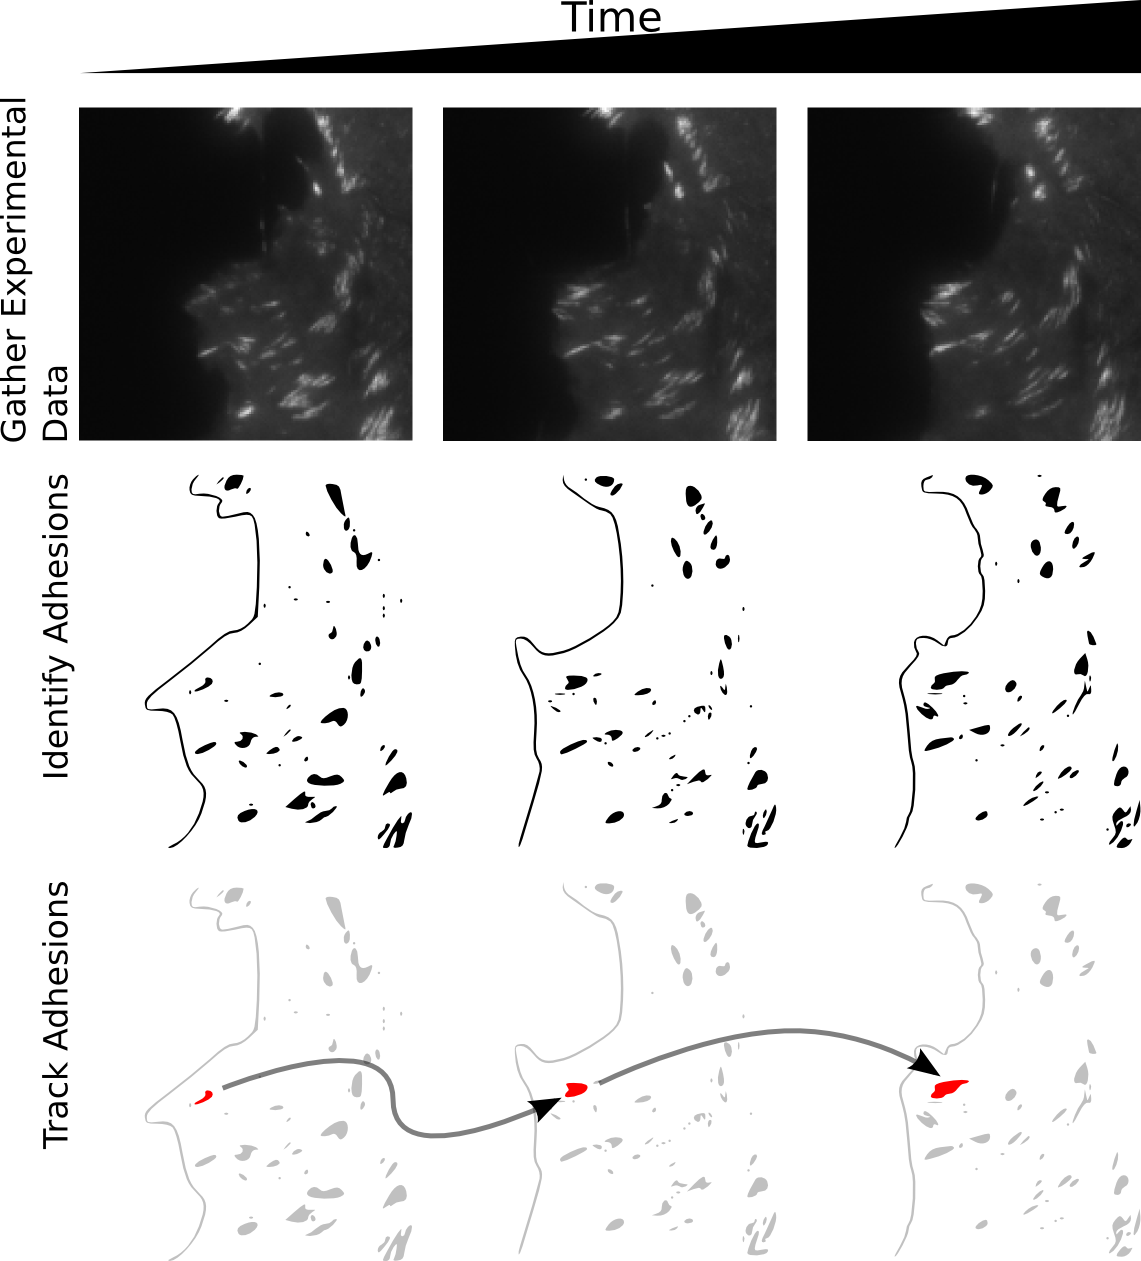
\includegraphics[width=\textwidth]{../figures/FA_workflow/graphic_workflow}
\end{center}
\caption{
{\bf Automating the analysis of focal adhesion images requires a multi-stage
pipeline.} The first row shows several representative example images of
fluorescently labeled Paxillin using TIRF micrscopy. These images only show a
small portion of the entire NIH 3T3 cell imaged in this experiment. In the
second row, a cartoon depiction of the segmented adhesions and the cell edge
are shown. Identification of the adhesions in each image allows a set of static
morphological and fluorescence intensity based features to be extracted. The
third row shows a single adhesion (highlighted in red) being tracked through
the short sample time course. While a single adhesion is highlighted in this
example, all the detected adhesions are tracked though each experiment. The
properties of each adhesion is tracked through time, allowing the large scale
dynamics of the focal adhesions to be determined.  
}
\label{method_flow}
\end{figure}

\begin{figure}[htbp]
\begin{center}
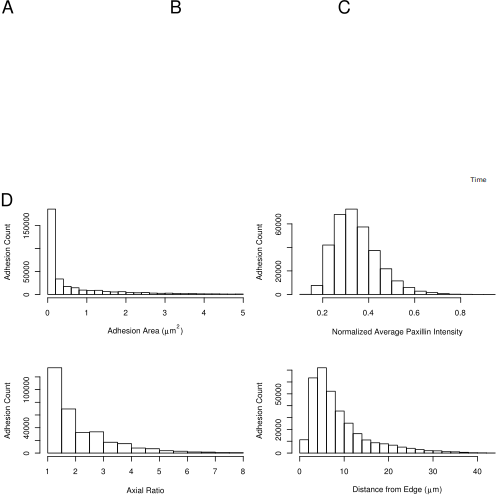
\includegraphics[width=0.8\textwidth]{../figures/statics/statics}
\end{center}
\caption{
{\bf Applying quantitative image processing methods to FA images allows
comprehensive characterization of FA properties.} (A) One frame from a 200
minute movie of NIH 3T3 cells expressing GFP-Paxillin (the scale bar represents
10 $\mu$m). (B) The same cell as in (A), with each adhesion outlined in a
different color. (C) The entire set of adhesions in an experiment can be
visualized by overlaying the adhesions from each microscopy image going from the
first image collected to the last image collected. This example includes the
adhesions from 198 images. (D) A large range of properties can be extracted from
the segmented FA, five samples are provided.  The area histogram was filtered to
only include adhesions with areas less than 5$\mu$m$^2$. The axial ratio
histogram was filtered to only include adhesions with an axial ratio of 8 or
less. The longevity histogram includes all adhesions, while the inset only
includes adhesions with longevity greater than 20. The histograms include data
from 21 cells.
}
\label{statics}
\end{figure}


\begin{figure}[htbp]
\begin{center}
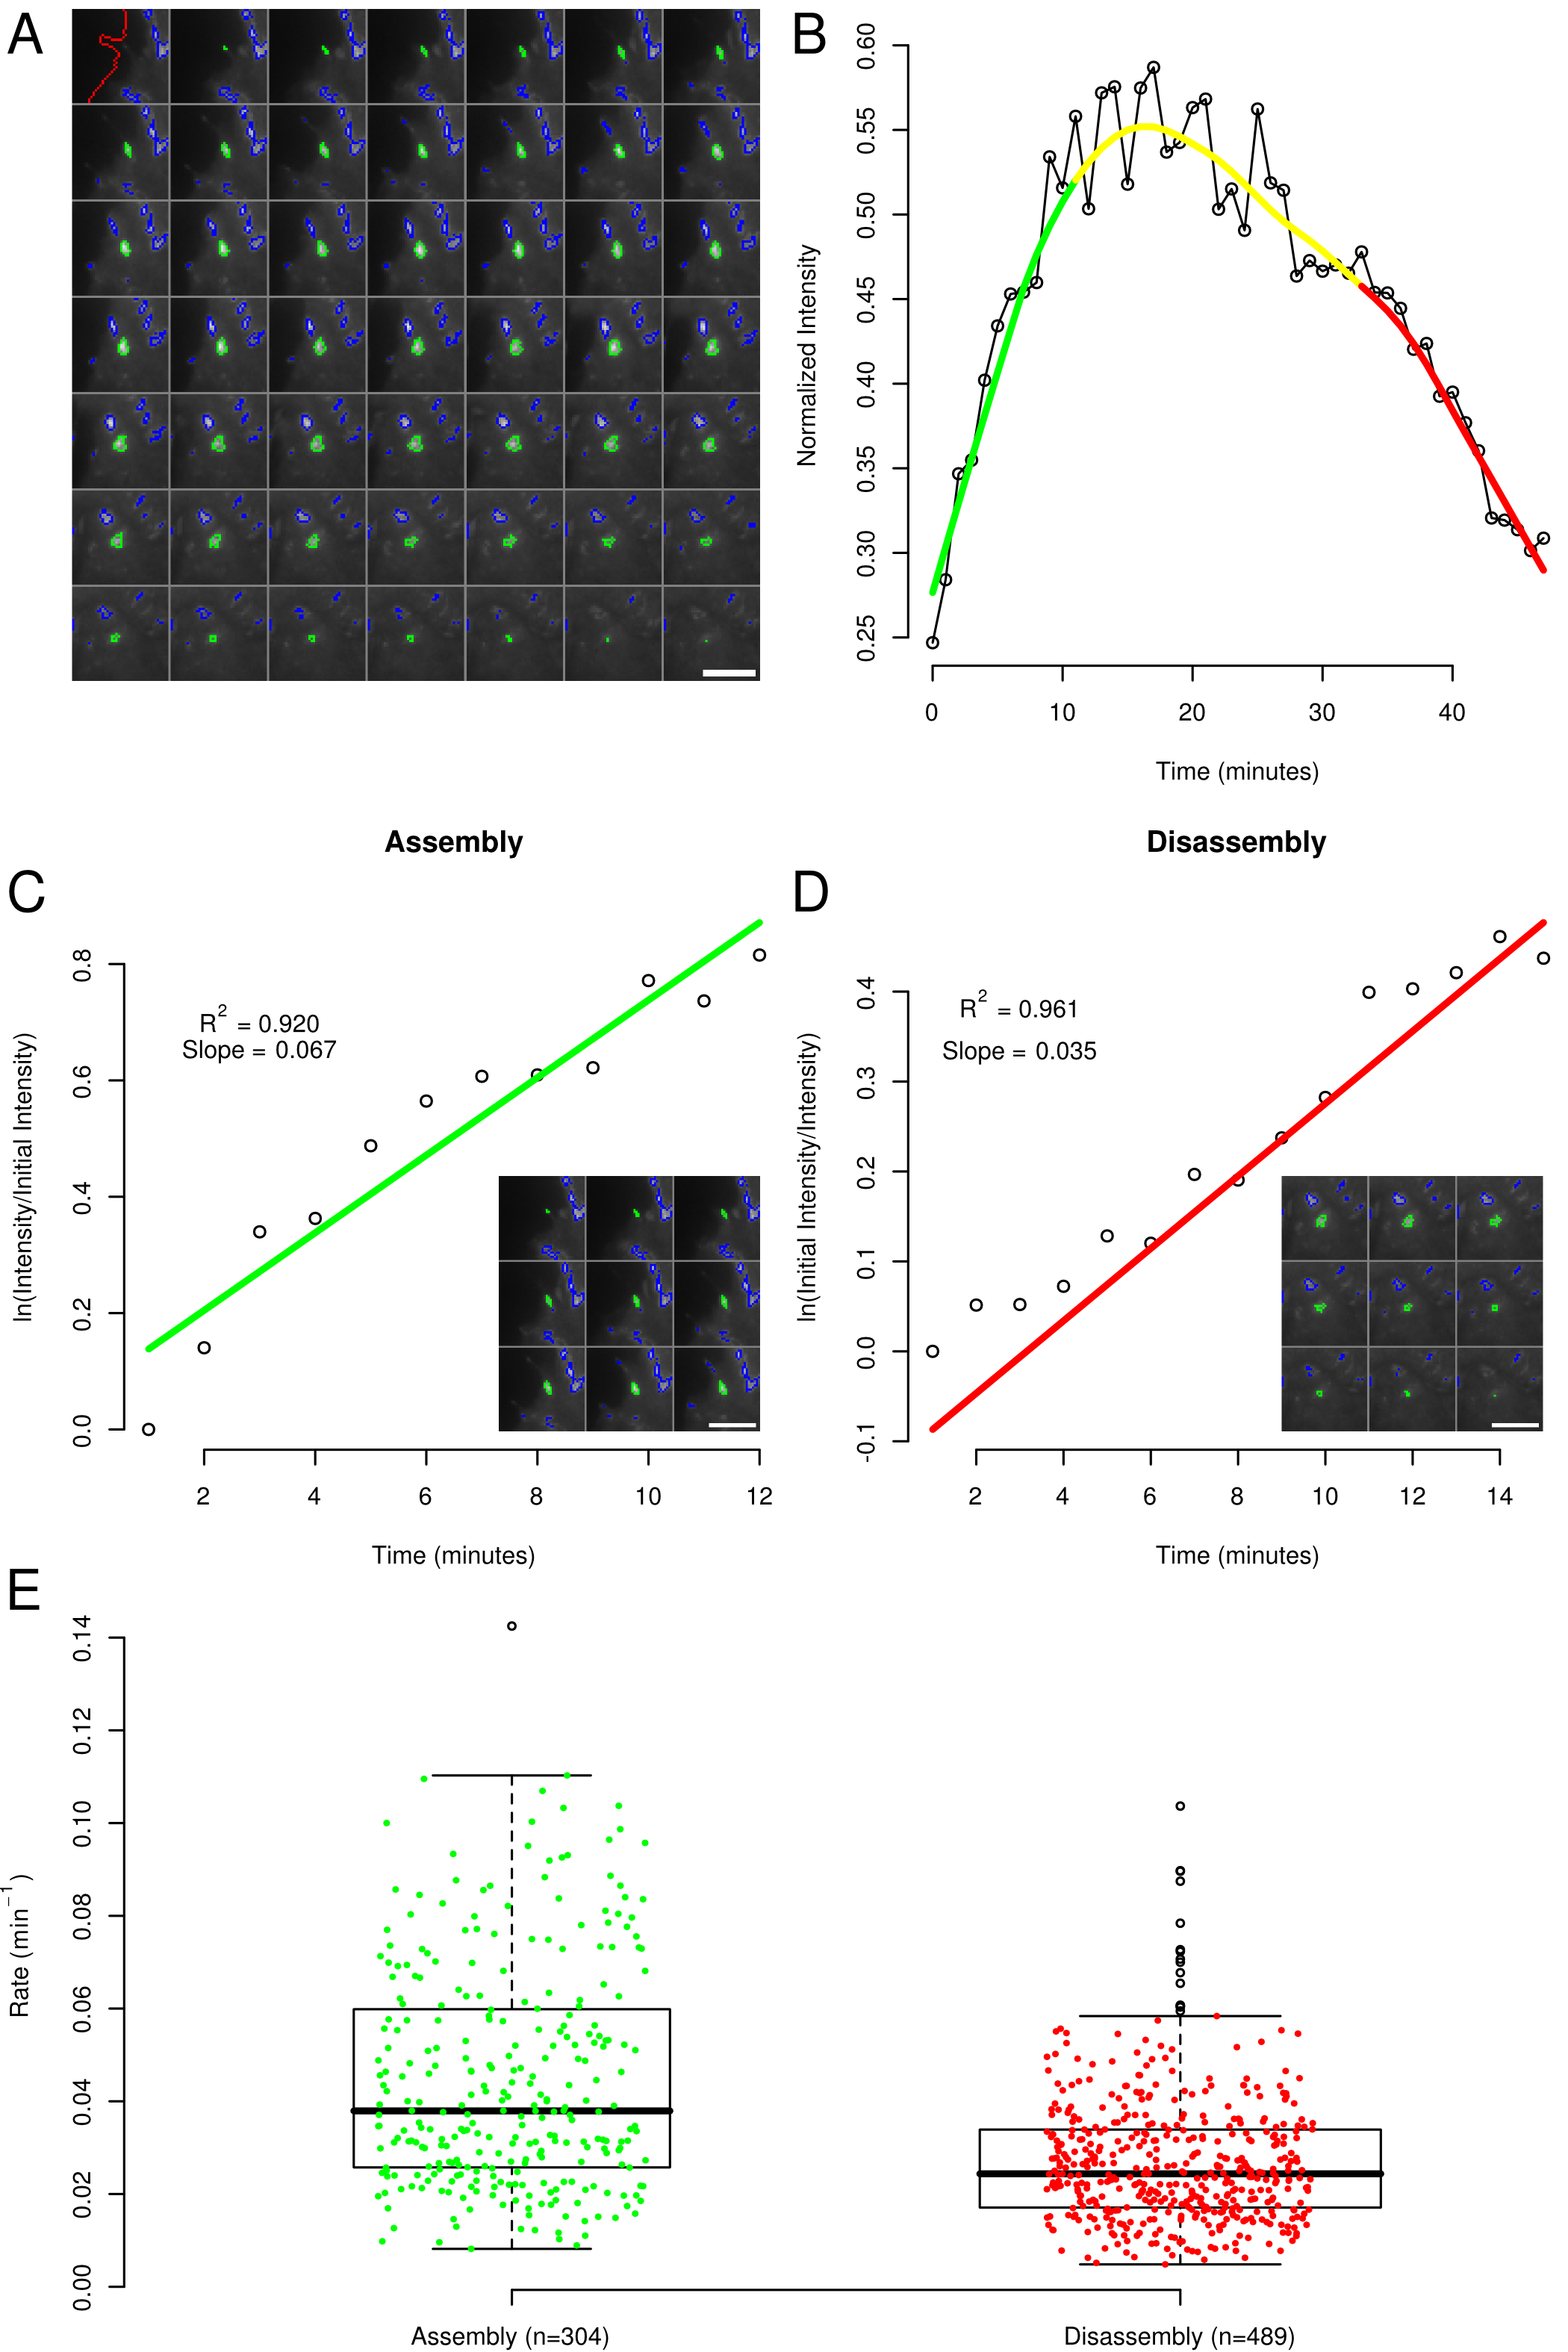
\includegraphics[height=0.8\textheight]{../figures/kinetics/kinetics}
\end{center}
\caption{
{\bf Focal adhesion kinetics.} (A) Each of the adhesions in the cells is
tracked, allowing the position and properties of single adhesions to be
assessed. Here a single adhesion (in green), the surrounding adhesions (in blue)
and the cell edge (in red) are followed for 49 minutes. The cell edge is only
outlined in the first frame. (B) The intensity of the paxillin in the tracked
adhesion in (A) through time. The red line is a smoothed fit to the data using
the lowess algorithm. (C) The normalized log-linear fit of the Paxillin
intensity through time during the assembly phase of the adhesion in part (B).
The inset depicts several of the images from which the Paxillin intensity was
gathered. The color highlights indicate the same cell features as in (A). (D)
The normalized log-linear fit of the Paxillin intensity through time during the
disassembly phase of the adhesion in part (B). The inset depicts several of the
images from which the Paxillin intensity was gathered. The color highlights
indicate the same cell features as in (A). (E) The assembly and disassembly
rates for adhesions whose Paxillin intensity curve fits have R$^2$ values of 0.9
or greater. The top and bottom lines of the boxplots indicate the 3$^\text{rd}$
and 1$^\text{st}$ quartiles respectively, while the bold lines indicate the
media values. The whiskers extend up to 1.5 times the interquartile range. The
scale bar is 10 $\mu$m.
}
\label{kinetics}
\end{figure}

\begin{figure}[htbp]
\begin{center}
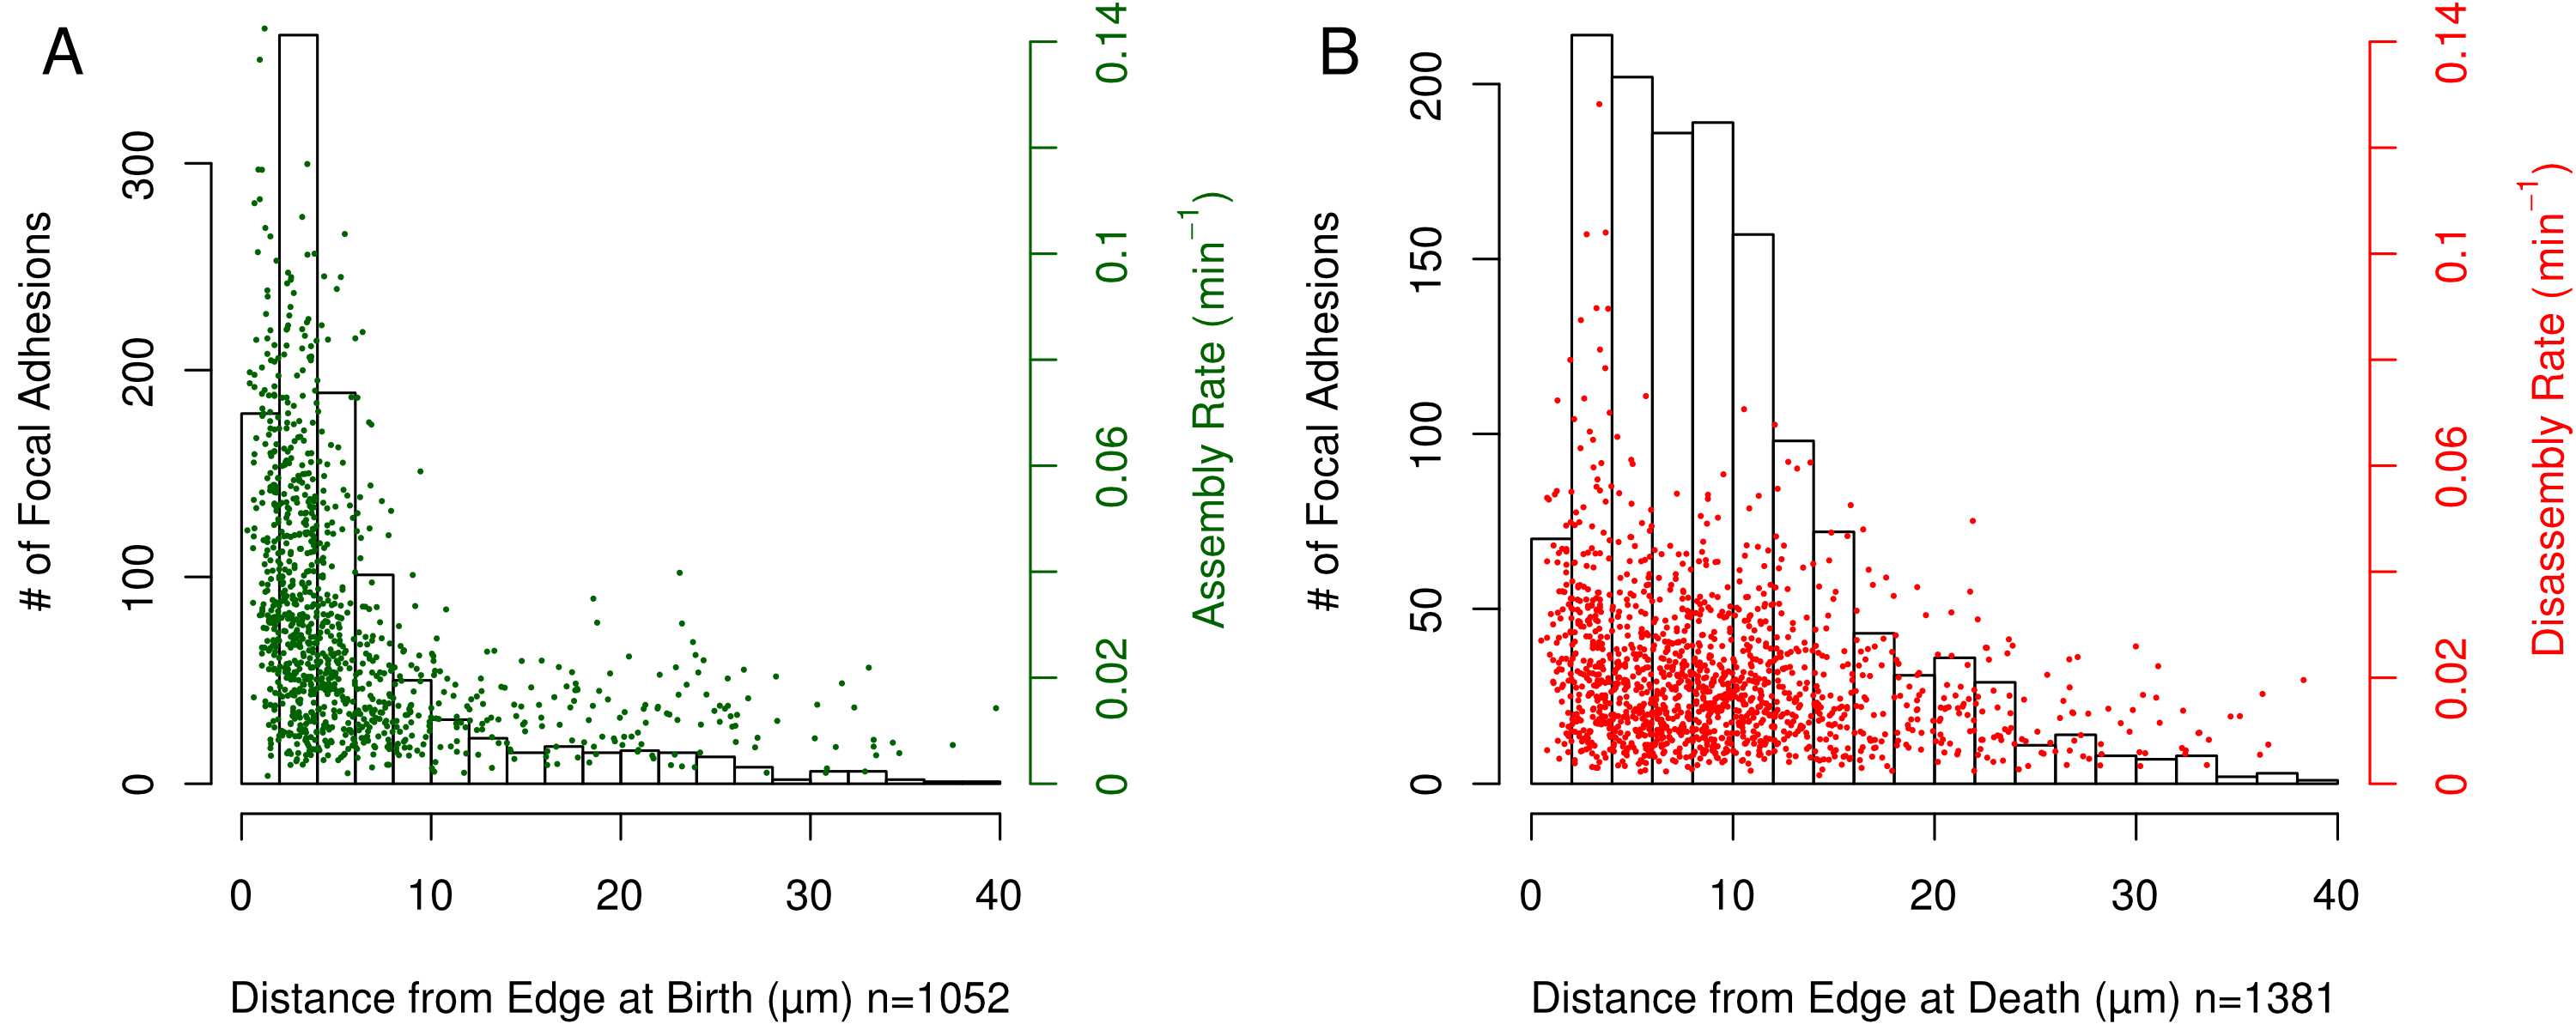
\includegraphics[width=\textwidth]{../figures/spatial/spatial}
\end{center}
\caption{
{\bf Spacial properties of FA centroid positions at birth and death where the
assembly and/or disassembly phases fit a log-linear model with R$^2$ value of
0.9 or greater.} (A) The majority of adhesions whose growth patterns demonstrate
a strong linear model are born within 5 $\mu$m of the cell edge. (B) The
distribution of the distance of death location from the cell edge indicates that
adhesion disassembly typically occurs along a broader band at the cell edge as
compared to the position at adhesion birth. (C) The variance of assembly rates
is greatest for adhesions born within $\sim$5 $\mu$m of the edge (D) The
variance of disassembly rates only has a slight decrease as the distance from
edge at death increases.  
}
\label{spatial}
\end{figure}

\begin{figure}[htbp]
\begin{center}
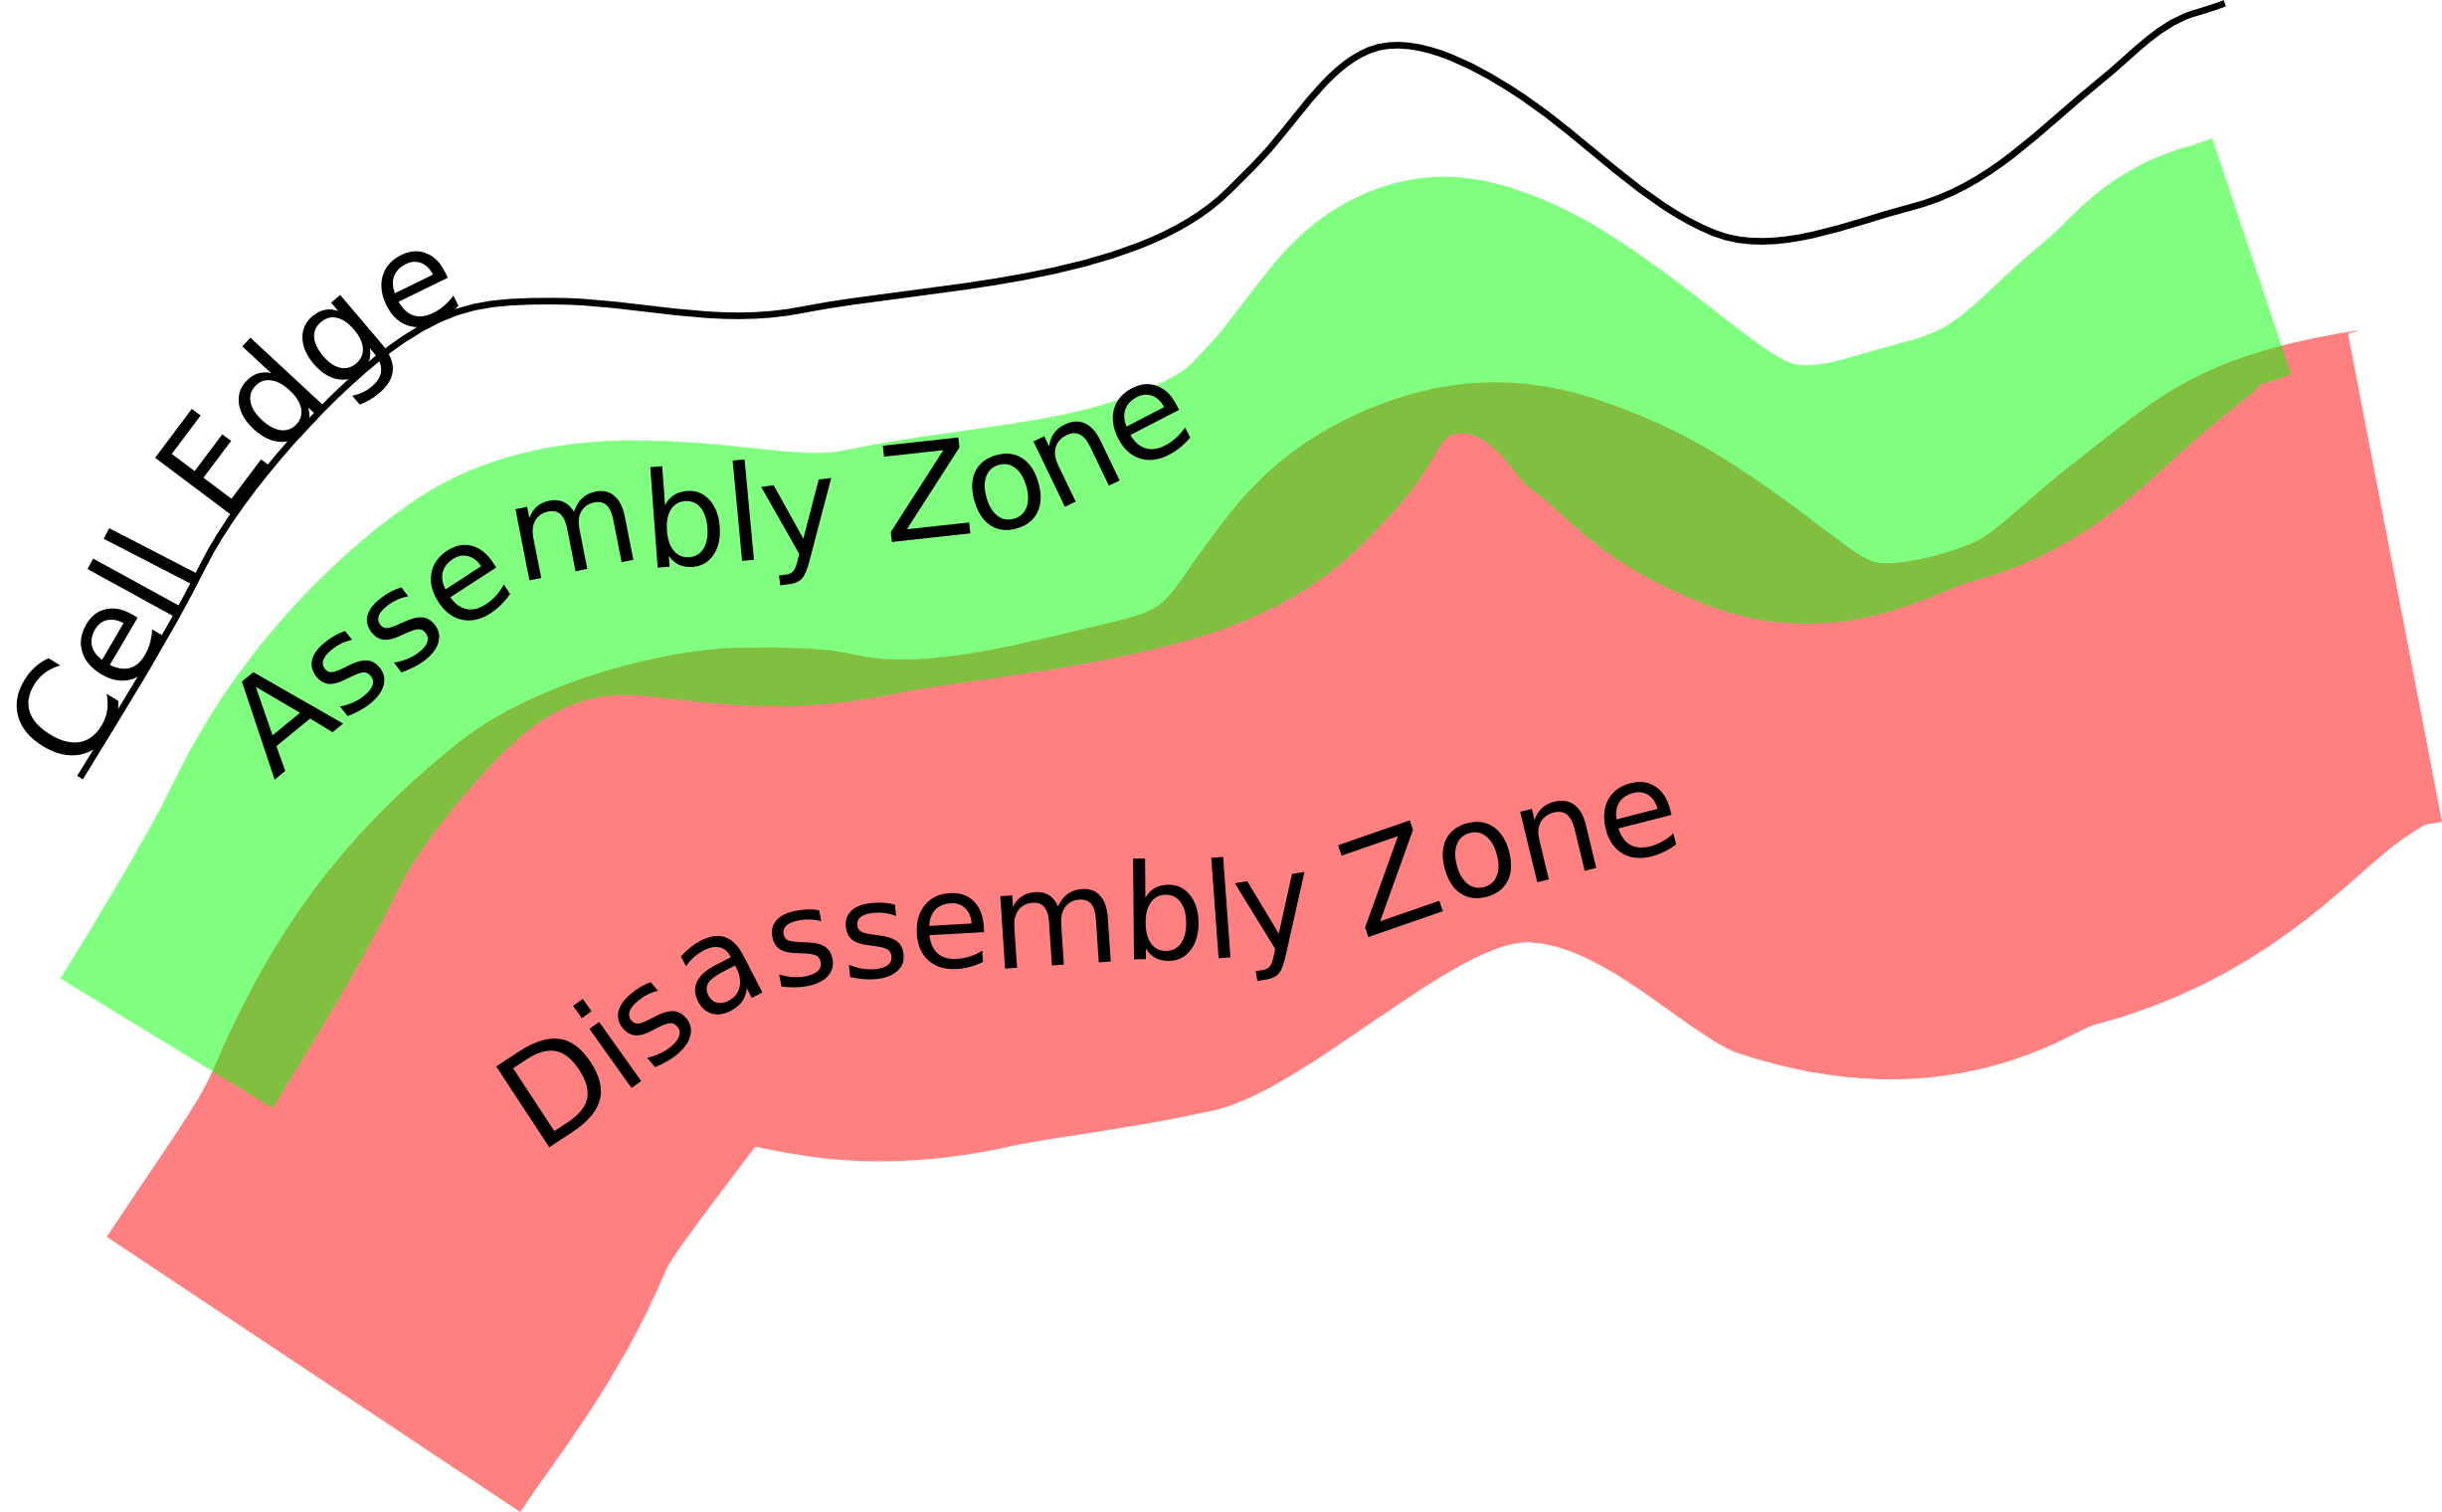
\includegraphics[width=0.5\textwidth]{../figures/spatial/cartoon}
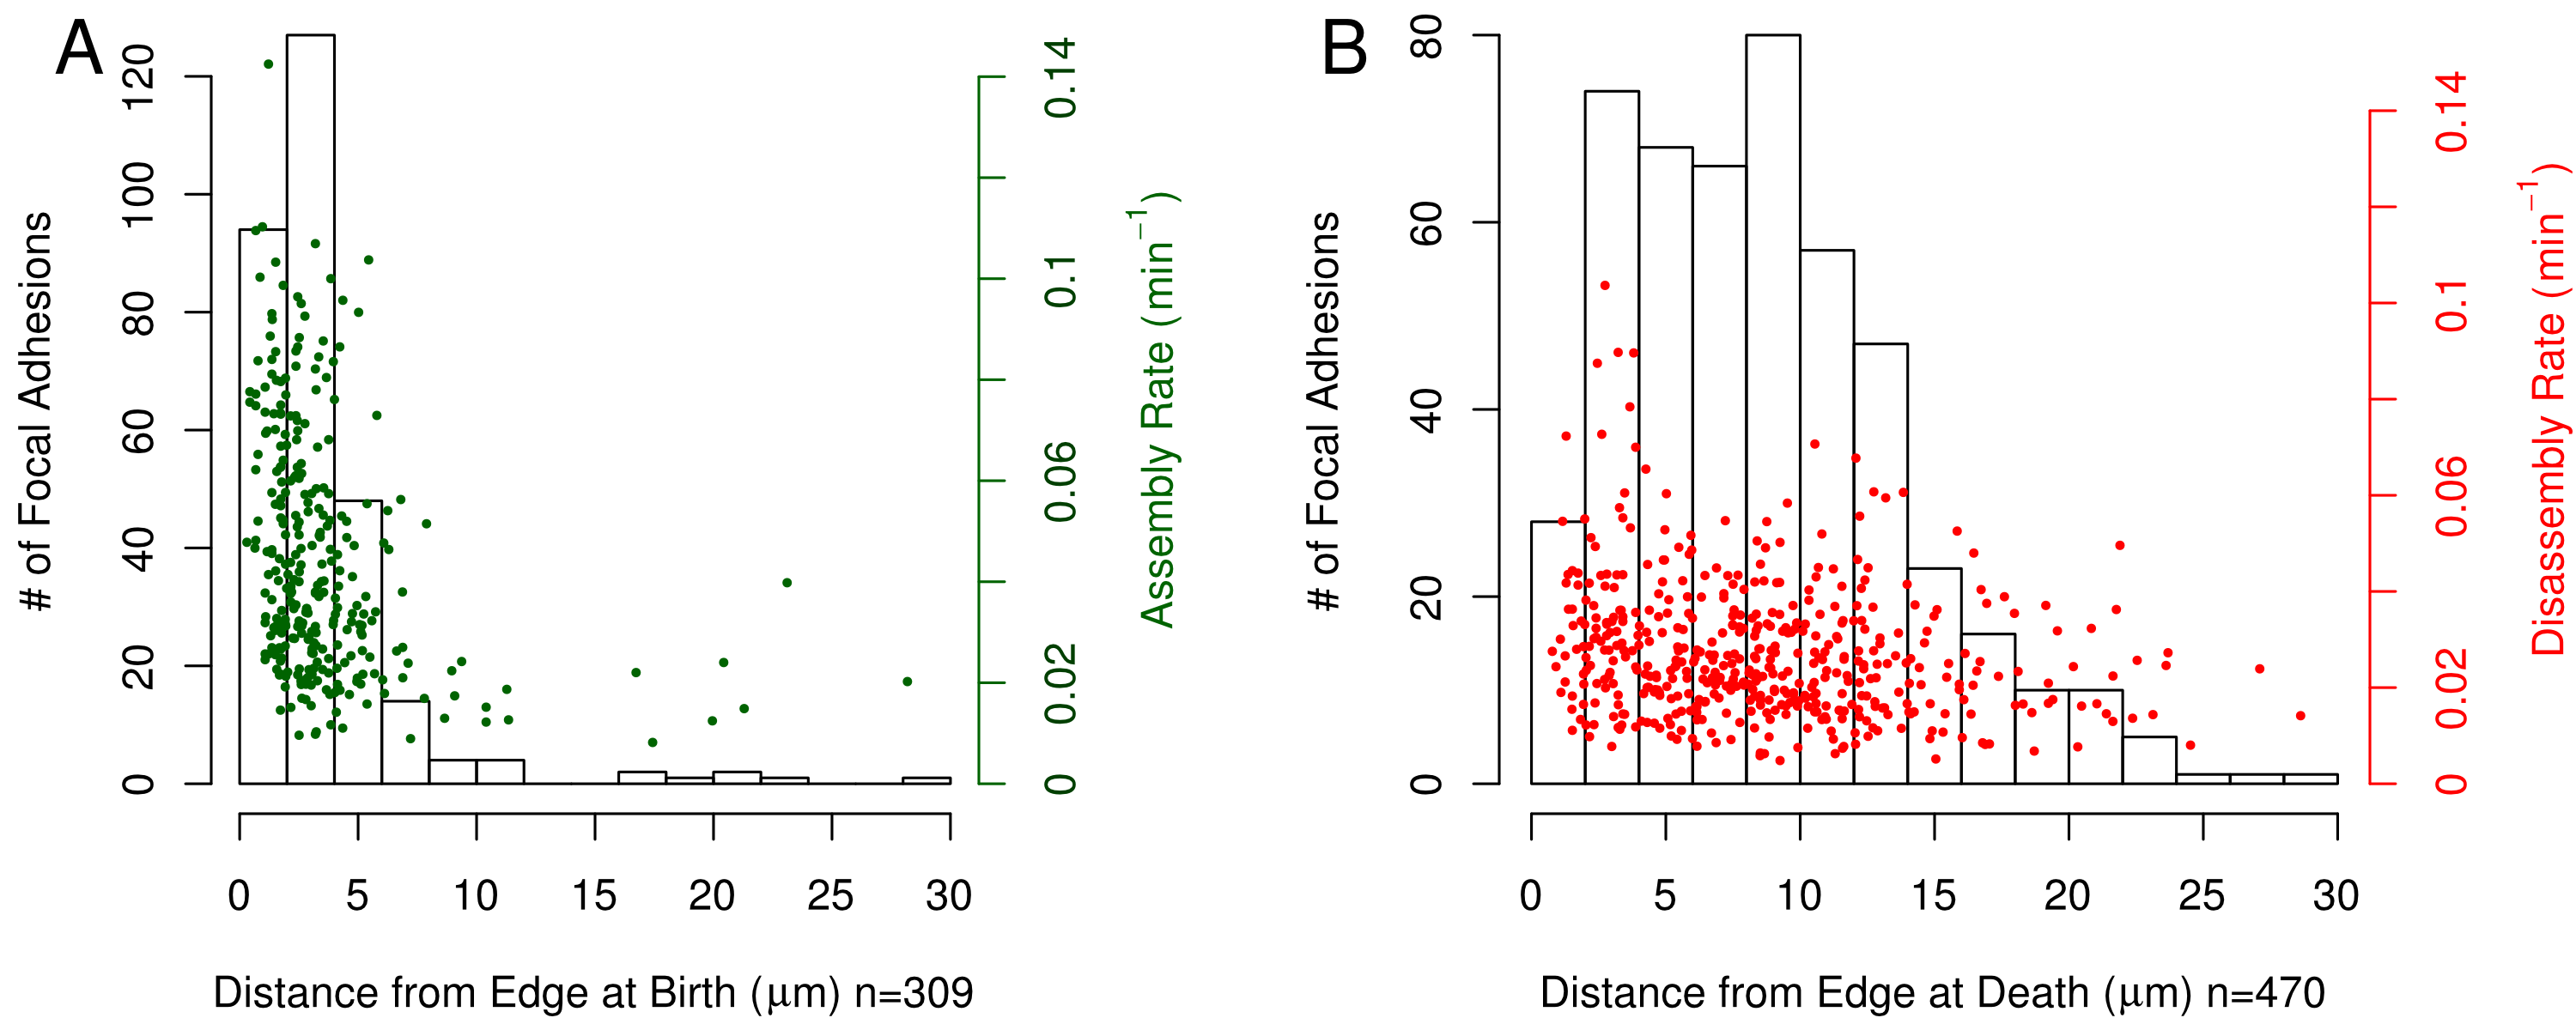
\includegraphics[width=\textwidth]{../figures/spatial/spatial_alt}
\end{center}
\caption{
{\bf Spacial properties alternative figure and cartoon.}
}
\label{spatial_alt}
\end{figure}

\begin{figure}[htbp]
\begin{center}
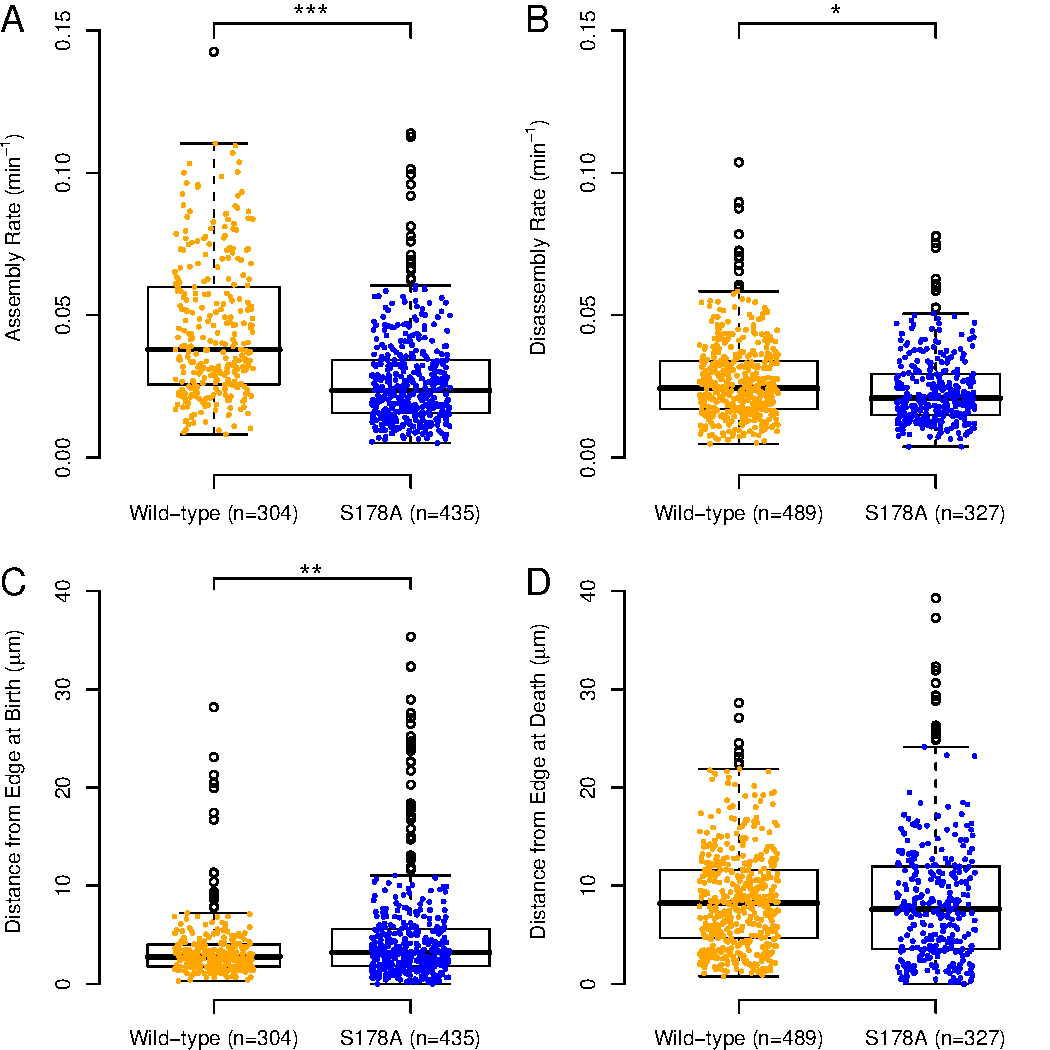
\includegraphics[width=\textwidth]{../figures/S178A/S178A_vs_wild-type}
\end{center}
\caption{
{\bf Comparison between several of the properties of the S178A mutants and
wild-type FA in adhesions which fit a log linear model with R$^2$ value of 0.9
or greater.} (A) The mean assembly rate is decreased by 40\% in the S178A case
(*** indicates $p<10^{-5}$). (B) The mean disassembly rate is also decreased,
but only by 16\% (** indicates $p<10^{-3}$). (C and D) The median position of
adhesion centroids at birth is increased by 44\% (** indicates $p<10^{-3}$),
while the median position of the adhesion centroid at death is unaffected in the
S178A mutants. All p-values were calculated using the bootstrapped
confidence intervals.  }
\label{S178A}
\end{figure}

\begin{figure}[htbp]
\begin{center}
\includegraphics[width=\textwidth]{../figures/lifetimes/adhesion_phase_lifetimes}
\end{center}
\caption{
{\bf The assembly and disassembly phases in S178A mutant FA are significantly
longer than those in the wild-type, while the stability phase lengths are
unaffected.} The phase length values include all adhesions where the log-linear
models fit with a p-value of 0.05 or less.  Error bars indicate 95\% confidence
intervals on the mean phase length as determined through 50,000 bootstrap
samples. A triple asterisk (***) indicates $p<10^{-5}$ and single asterisk (*)
indicates $p<0.05$. Wild-type N Values: Assembly (1057), Stability (456),
Disassembly (1371); S178A N Values: Assembly (2089), Stability (868),
Disassembly (1761)
}
\label{lifetimes}
\end{figure}

\begin{figure}[htbp]
\begin{center}
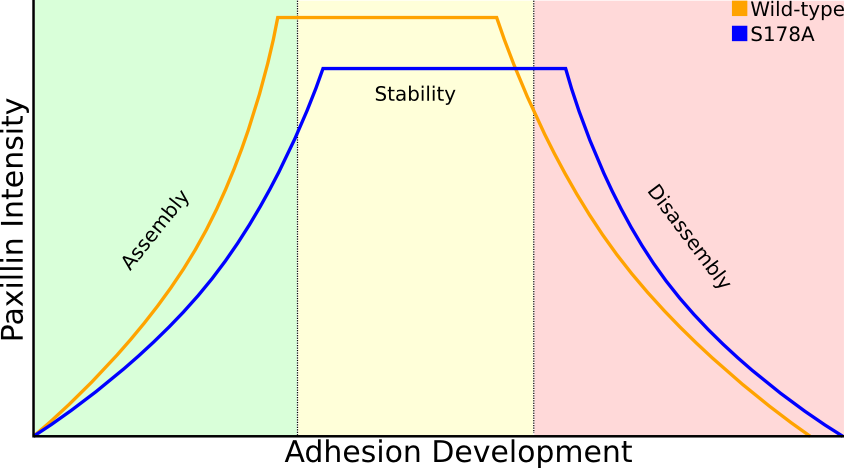
\includegraphics[width=\textwidth]{../figures/S178A/sample_timecourse}
\end{center}
\caption{
{\bf Mutations affecting the interaction of Jun Kinase with Paxillin modify all
stages of FA development.}  }
\label{summary}
\end{figure}


\section*{Tables}
\begin{table}[!ht]
\caption{
\bf{Properties Extracted}}
\begin{tabular}{cc|c}
Property Class & Name & Description\\
\hline
Static & FA Area & Total area covered by adhesion ($\mu$m$^2$)\\
 & FA Axial Ratio & Ratio between long and short axis of ellipsoid fit to the binary FA\\
 &Centroid Position & Location of binary adhesion centroid\\
 & Mean Fluorescence Intensity & Average normalized value of fluorescence intensity of each FA \\
 & Cell Area & Total area covered by cell ($\mu$m$^2$)\\
 & Distance from Cell Edge & Distance from nearest cell edge to adhesion centroid\\
\hline
Dynamic & Assembly Rate & Slope of normalized fluorescence intensity on a log scale versus time \\
 & Disassembly Rate & \\
 & Birth Position & Location where FA lineage starts\\
 & Length of Lifecycle Phases & Length of time spent in assembly, stability and disassembly\\
\end{tabular}
%\begin{flushleft}Table caption
%\end{flushleft}
\label{prop_table}
\end{table}

\end{document}
